\documentclass[12pt, a4paper]{article}
\usepackage[utf8]{inputenc}
\usepackage[IL2]{fontenc}
\usepackage[czech]{babel}
\usepackage{graphicx}

\begin{document}
\begin{figure}[h!]
\centering

\includegraphics[bb= 0 0 820 445 , width=75mm]{favlogo.jpg}
\end{figure}

\vspace{5cm}

{\centering
{\huge Architektura CRCE}\\[1em]
{\large KIV/SAR - semestrální práce}\\[7,5cm]
}

\begin{tabular}{l r}
student: & Radek VAIS, Zdeněk VALEŠ\\
mail: & vaisr@students.zcu.cz, valesz@students.zcu.cz\\
datum: & 1.1.2019\\
\end{tabular}

\thispagestyle{empty}
\newpage

%========================================
%========================================
%========================================
%========================================
%========================================
\section{Zadání} %=====================================================================================================

CRCE\footnote{Component Repository supporting Compatibility Evaluation} je komponentové úložiště vyvíjené v~rámci výzkumu na Katedře informatiky a výpočetní techniky na Západočeské univerzitě v~Plzni. Jeho hlavní vlastností je podpora kontroly kompatibility verzí různých OSGi komponent nebo webových api.

\subsection{Motivace}

Vývoj projektu probíhá již několik let a vystřídalo se na něm mnoho vývojářů, což způsobilo zanesení větších či menších architektonických dluhů. Projekt již můžeme klasifikovat jako velký. Existuje potřeba, aby střídající se vývojáři (např. v~rámci bakalářských prací) snadno a rychle zprovoznili základní instalaci a získali tak prostředí, pro rychlý vývoj nových částí. 

\subsection{Cíle projektu}

\begin{itemize}
	\item Unifikovat proces sestavení aplikace a spuštění.
	\item Zdokumentovat současnou architekturu aplikace.
	\item Analyzovat závislosti modulů v~projektu a ověřit, zda některé moduly mají být součástí jádra.
	\item Připravit Docker image pro vývojáře.
\end{itemize}

\newpage
%========================================
%========================================
%========================================
%========================================
%========================================
\section{Analýza~architektury} %============================================================================================

Celý projekt je rozdělen do čtyř hlavních modulů: sdílené nastavení sestavení, jádro, moduly a knihovny třetích stran. Ne zcela jasné je začlenění mechanismu pro nasazení a spuštění v~modulu \texttt{CRCE modules} (jedná se o~komponentu \texttt{provision}). Závislostí modulů na jádře pozorujeme dva typy. Prvním typem je závislost na agregačním modulu jádra, druhým je jmenovitá závislost na komponentách jádra. Tyto skutečnosti jsou patrné na celkovém diagramu na Obrázku \ref{fig:wholeCRCE}.

\begin{figure}[h!]
\centering
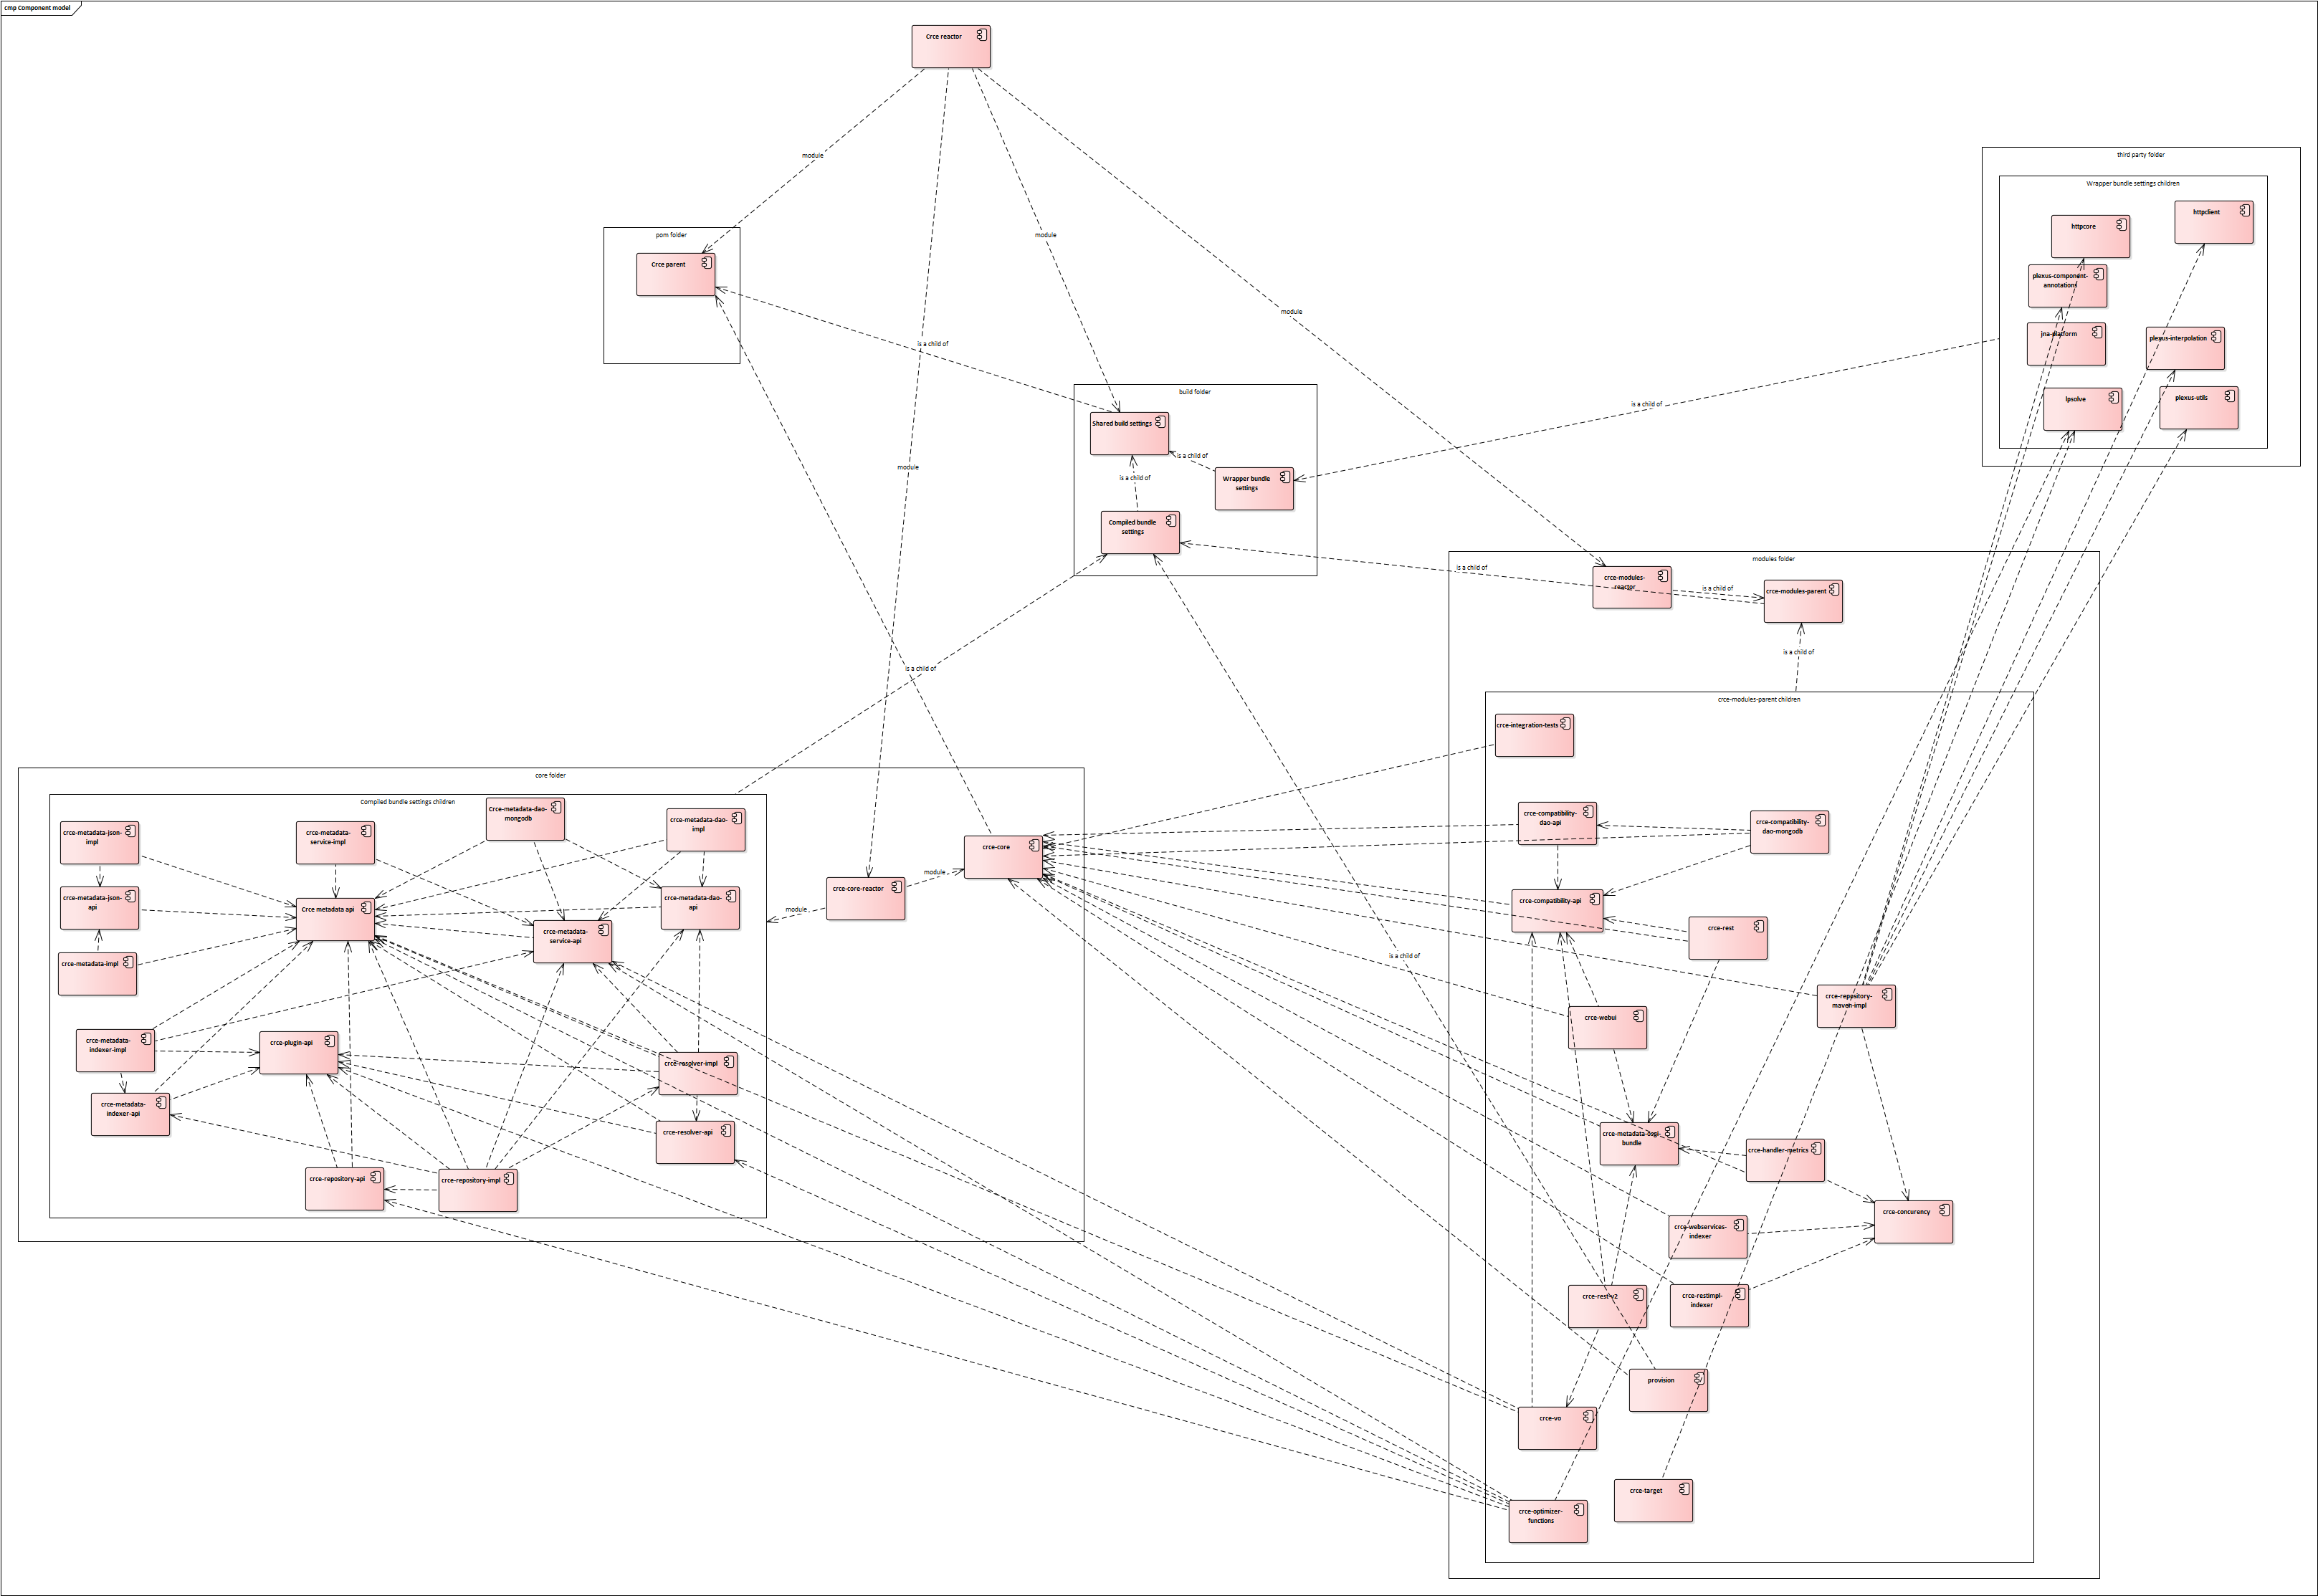
\includegraphics[width=135mm]{wholeCRCE.png}
\caption{Diagram závislostí všech maven komponent projektu CRCE před provedenými úpravami.}
\label{fig:wholeCRCE}
\end{figure}

Během analýzy modulu pro moduly CRCE jsme identifikovali několik kandidátů na přesun do jádra. Za kandidáty jsme volili takové komponenty, které využívá velká část ostatních modulů a zároveň tyto moduly mají závislosti do jádra. Komponenta webového rozhraní (\texttt{crce-webui}) tomuto pravidlu sice odporuje, představuje ale základní komponentu, bez které by úložiště nešlo použít. Přesouvané komponenty jsou: \texttt{crce-compatibility-api}, \texttt{crce-webui}, \texttt{crce-concurrency} (graficky znázorněno na Obrázku \ref{fig:modulesCRCE}). 

Po identifikaci kandidátů jsme z~přesunu vyřadili komponentu metadata-osgi-bundle, kvůli nedostatečné obecnosti. Komponenta je schopna indexovat pouze OSGI komponenty -- přesun do jádra by byl možný, pokud by uměla indexovat obecné JAR. Komponenta \texttt{crce-webui} bohužel obsahuje silnou závislost na této komponentě, která brání přesunu \texttt{crce-webui} do jádra. Závislost spočívá v~použití několika konstant, které jsou v~definované v~metadata-osgi-bundle. Navrhli jsme tedy přidání metody do rozhraní indexeru pro zjištění jaké elementy indexer zpracovává a silnou závislost jsme nahradili slabou závislostí.

\begin{figure}[h!]
\centering
\includegraphics[width=135mm]{modules.png}
\label{fig:modulesCRCE}
\caption{Diagram původních závislostí uvnitř modulu moduly CRCE. Zeleně jsou označeny přesouvané komponenty. Červeně je označena nevhodná závislost.}
\end{figure}

%========================================
%========================================
%========================================
%========================================
%========================================
\section{Provedené~změny} %=======================================================================================

V~projektu jsme provedli několik změn, které by měly vést k~zjednodušení práce budoucích vývojářů. Pro přehlednost dodávám, že v~této sekci pojem \textit{modul} značí maven modul v~kořenovém adresáři CRCE a pojem \textit{komponenta} značí jeden z~maven modulů obsahující konkrétní implementaci (\textit{crce-webui}, \textit{crce-metadata-api}, ...).

\subsection{Nový modul pro sestavení}
Do kořene CRCE byl přidán nový modul \textit{deploy}, do kterého byla přesunuta komponenta \textit{provision}, používaná ke spouštění CRCE. Jsou zde agregovány všechny komponenty z~jádra a komponenty z~modulu \textit{modules}, které jsou zachycené v~\textit{crce-default-modules}. 

Nově přidaná komponenta \textit{crce-default-modules} tedy slouží jako agregátor komponent z~modulu \textit{modules}, které mají být použité ve výsledné distribuci.

V~rámci přípravy modulu pro sestavení a spuštění byl přidán Docker image obsahující JDK 1.7 a Apache Felix verze 5.0.0.

\subsection{Přesun vybraných modulů do jádra}
Do jádra byly z~modulu \textit{modules} přesunuty komponenty: \textit{crce-compatibility-api}, \textit{crce-webui} a \textit{crce-concurrency}. V~případě \textit{crce-webui} bylo nutné odstranit závislost na \textit{crce-core} (jinak by se jednalo o~kruhovou závislost) a nahradit ji jednotlivými závislostmi na vybraných komponentách z~jádra.

V~komponentě \textit{crce-compatibility-api} bylo nutné přidat výchozí (prázdnou) implementaci rozhraní \textit{Compatibility} a \textit{Diff}. Pro tyto implementace byl přidán unit test.

Součástí přesunu komponent do jádra bylo přidání unit testu do \textit{crce-metadata-osgi-bundle}, který dokazuje schopnost této komponenty indexovat pouze OSGI bundly a ne obecné JAR.

\subsubsection{Nahrazení silné závislosti v~komponentě crce-webui}
Komponenta \textit{crce-webui} obsahovala silnou závislost na komponentě \textit{crce-metadata-osgi-bundle}. Tato závislost spočívala v~použití několika konstant, označujících indexované elementy, definovaných v~rozhraní \textit{NsOsgiIdentity}. Konstanty byly použity ve třídě \textit{ResourceServlet} k~filtrování zobrazovaných OSGI bundlů. 

Po dohodě s~vyučujícím jsme tuto závislost nahradili slabou závislostí -- konstanty stejného typu jsme dodefinovali i v~komponentě \textit{crce-webui}. Silná závislost byla odstraněna, nicméně pokud se v~budoucnu změní komponenta \textit{crce-metadata-osgi-bundle}, bude nutné kontrolovat, zda změna neovlivnila \textit{crce-webui} a případné nesrovnalosti opravit.

Aby bylo podobným závislostem v~budoucnosti zamezeno, rozhraní indexeru bylo rozšířeno o~metodu, která vrací elementy, jež je indexer schopen detekovat. V~rámci této práce byla vytvořena výchozí implementace této vlastnosti v~AbstractIndexer, která vrací pouze prázdný seznam. Projekt lze bezpečně přeložit, ale momentálně novou funkci rozhraní plně využívá jen OSGiIndexer.

\begin{figure}[h!]
\centering
\includegraphics[width=135mm]{indexerApi.png}
\label{fig:indexerApi}
\caption{Diagram ukazuje upravené rozhraní indexeru, které nově obsahuje metodu getIndexedAttributes, která slouží k~získání seznamu vlastností, které daný indexer zpracovává. Dále naznačuje možnost umístit implementaci indexeru do modulu crce-core nebo crce-modules (fiktivní indexery JarIndexer a AnotherIndexer).}
\end{figure}

\subsubsection{Načítání connection stringu}

Součástí příprav pro dockerizaci bylo přidání konfigurace připojení k~databázi MongoDB. Ke konfiguraci připojení lze nyní využít proměnnou prostředí \textit{mongo\_connection}, kde aplikace očekává MongoDB connection string\footnote{viz dokumentace: https://docs.mongodb.com/manual/reference/connection-string/}. V~případě, že tato proměnná není nastavena, použije se výchozí hodnota (\textit{mongodb://localhost:27017}, která nese připojení k~databázi běžící na localhostu a standardním portu. Výhodou tohoto přístupu je možnost konfigurovat connection string v~Dockerfile a při změně pouze znovu sestavit image.


\section{Dockerizace projektu}
Do modulu \textit{deploy} byl přidán Dockerfile, kterým je možné sestavit docker image obsahující spustitelnou verzi CRCE. Do takto spuštěného CRCE lze doinstalovávat nové OSGi komponenty a není nutné celý projekt znovu sestavovat. 

Detaily o~sestavení a spuštění docker image jsou v~sekci \ref{sec:manual}

%========================================
%========================================
%========================================
%========================================
%========================================
\section{Uživatelská~příručka}
\label{sec:manual} %======================================================================================

Provedené změny ovlivnily základní používání projektu při vývoji. 

Pro sestavení na platformě Linux lze použít bash script \textit{build.bash}\footnote{Teoreticky není nutná platforma Linux. Pro uživatele Windows by měl být dostačující bash interpret nebo Linux subsystem. Tato možnost nebyla testována.}, který automaticky spustí jednotlivé kroky sestavení pomocí nástroje Maven. Script vždy vykonává všechny kroky od začátku, v~případě selhání je vhodné po opravě pokračovat v~buildu manuálně.

V~případě, že databáze neběží na localhostu, nebo standardním portu, je možné nastavit připojení skrze proměnnou prostředí \textit{mongo\_connection}. Tato proměnná by v~případě použití měla obsahovat celý connection string. Pokud není nastavená, pro připojení k~databázi bude použita výchozí hodnota: \textit{mongodb://localhost:27017}.

\subsection{Docker}
K~sestavení Docker image je možné použít Dockerfile, který se nachází v~modulu \textit{deploy}. Sestavení image je provedeno příkazem:

\begin{verbatim}
docker build . -t crce-docker
\end{verbatim} 

\subsection{Spuštění docker image}

Výsledný image obsahuje distribuci Apache Felix 5.0.0, JDK 1.7 a všechny OSGI bundly z~CRCE. Spuštění lze provést příkazem:

\begin{verbatim}
docker run -it \ 
	   -p 8080:8080 \
	   --add-host mongoserver:172.17.0.1 \
	   -v /felix/deploy:/felix/felix-framework-5.0.0/dist \
	   crce-docker 
\end{verbatim}

Parametry \textit{-it} spustí image v interaktivním módu a přesměrují do něj STDIN. Tím je možné používat interaktivní GoGo shell. Pokud budou tyto parametry vynechány, GoGo shell nebude schopný detekovat žádný vstup a automaticky vypne běžící Felix.

Parametr \textit{--add-host} slouží k přidání záznamu do /etc/hosts v kontejneru a image se pak může k databázi běžící na hostujícím stroji připojit pomocí hostname \textit{mongoserver}. 

IP 172.17.0.1 je adresa, kterou docker přiřazuje hostujícímu stroji. Do adresáře \textit{/felix/deploy} na hostujícím stroji je možné vložit OSGI bundly a ty následně nainstalovat a spustit skrze Gogo shell. K~běžící instanci je možné přistoupit na adrese \textit{http://localhost:8080/crce}. 

Parametr \textit{-v} slouží k propojení adresáře na hostujícím stroji (\textit{/felix/deploy}) s adresářem uvnitř kontejneru (\textit{/felix/felix-framework-5.0.0/dist}). Do tohoto adresáře je možné kopírovat OSGI bundly a instalovat je v runtime.

Před spuštěním docker image je třeba spustit instanci MongoDB. Není podstatné, zda bude spuštěna prostřednictvím Dockeru (např. image 3.4-jessie), lokálním stroji nebo na serveru. Jen je třeba před sestavením ověřit nastavení connection string. Není připravena konfigurace docker-compose, protože se nám v~rámci konfigurace a testů nepodařilo zprovoznit GoGo shell při použití compose mechanismu, z~toho důvodu by uživatel byl ochuzen o~diagnostické možnosti OSGi runtime.


\subsection{Možné problémy při spuštění}
Pokud není spuštěný docker daemon, nebo současný uživatel není ve skupině \textit{docker}, může příkaz \verb|docker run| vyžadovat spuštění pod rootem \footnote{Kroky po nainstalování dockeru: https://docs.docker.com/install/linux/linux-postinstall/}.

V~případě, že by IP 172.17.0.1 nefungovala, je potřeba zjistit pod jakou adresou vidí docker hostující stroj. Ve výchozím nastavení vytvoří docker síťový most \verb|docker0| mezi imagem a hostujícím strojem. Detaily mostu lze zobrazit příkazem: 

\begin{verbatim}
sudo ip addr show docker0
\end{verbatim}

IP zobrazená ve výstupu příkazu je adresa, pod kterou docker container vidí hostovací stroj\footnote{Více detailů zde: https://stackoverflow.com/questions/24319662/from-inside-of-a-docker-container-how-do-i-connect-to-the-localhost-of-the-mach}.

%========================================
%========================================
%========================================
%========================================
%========================================
\newpage
\section{Závěr}  %======================================================================================================

V~rámci projektu jsme naplnili cíl usnadnit novým vývojářům spuštění výchozí aplikace, především přípravou docker image. Nepodařilo se nám zjednodušit proces sestavení celé aplikace na jeden Maven příkaz nicméně pro prostředí Linux jsme vytvořili script, který úkony nutné pro sestavení provede automaticky.
Dále jsme přesunuli několik modulů do jádra CRCE z~důvodu jejich provázanosti s~ostatními nebo nutnosti pro používání. 


\end{document}